\documentclass[12pt,a4paper]{article}

\usepackage[utf8]{inputenc}
\usepackage[T1]{fontenc}
\usepackage[swedish]{babel}
\usepackage{amsmath}
\usepackage{ae}
\usepackage{units}
\usepackage{icomma}
\usepackage{color}
\usepackage{graphicx}
\usepackage{bbm}
\usepackage{wrapfig}
%\usepackage{epsfig}
\usepackage[retainorgcmds]{IEEEtrantools}
\usepackage{hyperref}
\hypersetup{colorlinks,
	citecolor=black,
	filecolor=black,
	linkcolor=black,
	urlcolor=black,
	pdftex}
\newcommand{\N}{\ensuremath{\mathbbm{N}}}
\newcommand{\Z}{\ensuremath{\mathbbm{Z}}}
\newcommand{\Q}{\ensuremath{\mathbbm{Q}}}
\newcommand{\R}{\ensuremath{\mathbbm{R}}}
\newcommand{\C}{\ensuremath{\mathbbm{C}}}
\newcommand{\rd}{\ensuremath{\mathrm{d}}}
\newcommand{\id}{\ensuremath{\,\rd}}
\newcommand{\degree}{\ensuremath{^{\circ}}}


\begin{document}
	\pagenumbering{roman}

\title{Analytisk och nummerisk undersökning av modell för oscillerande partiklar upphängda i ideala fjädrar i en spatiell dimension}
	\author{Stefan Buller och Martin Wernstål}
	\date{DATE}
	\maketitle{}
	\thispagestyle{empty}

	\begin{abstract}
		Sammanfattning
	\end{abstract}

\newpage{}

	\tableofcontents{}
	\thispagestyle{empty}

\newpage{}

	\setcounter{page}{1}
	\pagestyle{plain}
	\pagenumbering{arabic}
	
	
\section{Problem 1}
	
	\setlength{\unitlength}{1mm}
	\begin{picture} (120, 40)
		\put(25, 20){\circle{20}}
		\put(57, 20){\circle{20}}
		\put(89, 20){\circle{20}}
		
		\put(0, 20){\line(5,0){5}}
		\put(5, 20){\line(1,5){1}}
		\put(6, 25){\line(1,-5){1}}
		\put(7, 20){\line(1,-5){1}}
		\put(8, 15){\line(1,5){1}}
		\put(9, 20){\line(1,5){1}}
		\put(10, 25){\line(1,-5){1}}
		\put(11, 20){\line(1,-5){1}}
		\put(12, 15){\line(1,5){1}}
		\put(13, 20){\line(5,0){5}}
		
		\put(32, 20){\line(5,0){5}}
		\put(37, 20){\line(1,5){1}}
		\put(38, 25){\line(1,-5){1}}
		\put(39, 20){\line(1,-5){1}}
		\put(40, 15){\line(1,5){1}}
		\put(41, 20){\line(1,5){1}}
		\put(42, 25){\line(1,-5){1}}
		\put(43, 20){\line(1,-5){1}}
		\put(44, 15){\line(1,5){1}}
		\put(45, 20){\line(5,0){5}}
		
		\put(64, 20){\line(5,0){5}}
		\put(69, 20){\line(1,5){1}}
		\put(70, 25){\line(1,-5){1}}
		\put(71, 20){\line(1,-5){1}}
		\put(72, 15){\line(1,5){1}}
		\put(73, 20){\line(1,5){1}}
		\put(74, 25){\line(1,-5){1}}
		\put(75, 20){\line(1,-5){1}}
		\put(76, 15){\line(1,5){1}}
		\put(77, 20){\line(5,0){5}}
		
		\put(96, 20){\line(5,0){5}}
		\put(101, 20){\line(1,5){1}}
		\put(102, 25){\line(1,-5){1}}
		\put(103, 20){\line(1,-5){1}}
		\put(104, 15){\line(1,5){1}}
		\put(105, 20){\line(1,5){1}}
		\put(106, 25){\line(1,-5){1}}
		\put(107, 20){\line(1,-5){1}}
		\put(108, 15){\line(1,5){1}}
		\put(109, 20){\line(5,0){5}}
		
		\put(23, 19){$m$}
		\put(55, 19){$m$}
		\put(87, 19){$m$}
		
		\put(8, 27){$k$}
		\put(40, 27){$k$}
		\put(72, 27){$k$}
		\put(104, 27){$k$}
		
	\end{picture}
	
	\setlength{\unitlength}{1mm}
	\begin{picture} (120, 40)
		\put(25, 20){\circle{20}}
		\put(57, 20){\circle{20}}
		\put(89, 20){\circle{20}}
		
		\put(18, 20){\vector(-1,0){8}}
		
		\put(32, 20){\vector(1,0){8}}
		
		\put(50, 20){\vector(-1,0){8}}
		
		\put(64, 20){\vector(1,0){8}}
		
		\put(82, 20){\vector(-1,0){8}}
		
		\put(96, 20){\vector(1,0){8}}
		
		\put(23, 19){$m$}
		\put(55, 19){$m$}
		\put(87, 19){$m$}
		
		\put(10, 22){$kq_1$}
		\put(32.5, 22){$k(q_2-q_1)$}
		\put(64.5, 22){$k(q_3-q_2)$}
		\put(98, 22){$-k(q_3)$}
		
		\put(25, 30){\line(0,1){2}}
		\put(57, 30){\line(0,1){2}}
		\put(89, 30){\line(0,1){2}}
		
		\put(25, 31){\vector(1,0){8}}
		\put(57, 31){\vector(1,0){8}}
		\put(89, 31){\vector(1,0){8}}
		
		\put(27, 33){$q_1$}
		\put(59, 33){$q_2$}
		\put(91, 33){$q_3$}
		
	\end{picture}

	Ur friläggning av de enskilda partiklarna finner vi att:

	\begin{IEEEeqnarray*}{rCl}
		m \ddot{q_1} & = & k (q_2 - q_1) - kq_1 \\
		m \ddot{q_2} & = & k (q_3 - q_2) - k (q_2 - q_1) \\
		m \ddot{q_3} & = & k (q_3 - q_2) - kq_3
	\end{IEEEeqnarray*}

	Vilket är ekvivalent med:

	\begin{IEEEeqnarray*}{rCrCrCrCl}
		\ddot{q_1} &+& \frac{2k}{m}q_1 &-& \frac{k}{m}q_2 & & & = & 0 \\
		\ddot{q_2} &-& \frac{2}{m}q_1 &+& \frac{2k}{m}q_2 &-& \frac{k}{m}q_3 &=& 0 \\
		\ddot{q_3} & & &-&\frac{k}{m}q_2 &+&\frac{2k}{m}q_3 & = & 0
	\end{IEEEeqnarray*}
	
	Vi inför beteckningarna: 

	\begin{IEEEeqnarray*}{rClCrClCrCl}
		\omega_o & = & \sqrt{k/m} &\hspace{12pt} &
		K & = &
		\begin{bmatrix}
			2  & -1 &  0 \\
 			-1 & 2  & -1 \\
 			0  & -1 &  2
		\end{bmatrix} &\hspace{12pt}&
		Q &=&
		\begin{bmatrix}
			q_1 \\ 
			q_2 \\
			q_3
		\end{bmatrix}
	\end{IEEEeqnarray*}

	Vårt system av differentialekvationer kan nu skrivas som:

	\begin{equation*}
		\ddot{Q} + \omega_o^2 KQ = 0
	\end{equation*}

	Vi gör ansatzen:

	\begin{IEEEeqnarray*}{rClCrCl}
		Q(t) & = & A e^{i \omega t} &\hspace{12pt}&
		A & = &
		\begin{bmatrix}
			a_1 \\
			a_2 \\
			a_3
		\end{bmatrix}
	\end{IEEEeqnarray*}

	Där $a_i, i = 1,2,3$ är amplituder för respektive partikel. Vilket ger oss:

	\begin{IEEEeqnarray}{rCl}
		\ddot{Q}&=&-\omega^2 A e^{i \omega{} t}
		\label{qdprick}
	\end{IEEEeqnarray}

	Och insatt i ekvationssystemet får vi:

	\begin{IEEEeqnarray*}{l}
	 	e^{i \omega t}(-\omega^2 A + \omega_o^2 K A) = 0
		\hspace{6pt}
		\Leftrightarrow
		\hspace{6pt}
		KA  = \frac{\omega^2}{\omega_o^2} A
	\end{IEEEeqnarray*}

	Detta känns igen som ett egenvärdesproblem. Genom att betrakta den karakteristiska ekvationen:
	\begin{IEEEeqnarray*}{rrCl}
	&	\begin{vmatrix}
			2-\frac{\omega^2}{\omega_o^2} & -1 & 0\\
			-1 & 2 - \frac{\omega^2}{\omega_o^2} & -1 \\
			0 & -1 & 2 - \frac{\omega^2}{\omega_o^2}
		\end{vmatrix} & = & 0 \\
		\Leftrightarrow &{\frac{\omega^2}{\omega_o^2}}^3 - 6 {\frac{\omega^2}{\omega_o^2}}^2 + 10 \frac{\omega^2}{\omega_o^2} - 4 & = & 0
	\end{IEEEeqnarray*}

	finner vi att egenvärdena är:

	\begin{IEEEeqnarray*}{C}
		\begin{cases}
			\frac{\omega_1^2}{\omega_o^2}=2 \\
			\frac{\omega_2^2}{\omega_o^2}=2+\sqrt{2} \\
			\frac{\omega_3^2}{\omega_o^2}=2-\sqrt{2} 
		\end{cases}
		\Leftrightarrow{}
		\hspace{12pt}
		\begin{cases}
			\omega_1 = \sqrt{2} \omega_o \\
			\omega_2 = \Big(\sqrt{2+\sqrt{2}}\Big) \omega_o \\
			\omega_3 = \Big(\sqrt{2-\sqrt{2}}\Big) \omega_o
		\end{cases}
	\end{IEEEeqnarray*}

	Genom att betrakta $(K-\frac{\omega_i^2}{\omega_o^2}I)A_i=0$ för $i=1,2,3$ finner vi egenvektorerna:
	
	\begin{IEEEeqnarray*}{rClCrClCrCl}
		A_1&=&
		\begin{bmatrix}
			1 \\ 
			0 \\
			-1
		\end{bmatrix} &\hspace{12pt}&
		A_2&=&
		\begin{bmatrix}
			1 \\
			-\sqrt{2} \\
			1 
		\end{bmatrix} &\hspace{12pt}&
		A_3&=&
		\begin{bmatrix}
			1 \\
			\sqrt{2} \\
			1
		\end{bmatrix}
	\end{IEEEeqnarray*}
	
	Vilket kan normaliseras till en ON-bas för $\R^3$:

	\begin{IEEEeqnarray*}{rClrClrCl}
		\hat{A_1} & = & \frac{1}{\sqrt{2}}
		\begin{bmatrix}
			1 \\ 
			0 \\
			-1
		\end{bmatrix} & \hspace{12pt}
		\hat{A_2} & = & \frac{1}{2}
		\begin{bmatrix}
			1 \\
			-\sqrt{2} \\
			1 
		\end{bmatrix} & \hspace{12pt}
		\hat{A_3} & = & \frac{1}{2}
		\begin{bmatrix}
			1 \\
			\sqrt{2} \\
			1
		\end{bmatrix}
	\end{IEEEeqnarray*} 
%Då vi har 3 distinkta egenvärden vet vi att våra 3 egenvektorer är ortogonala, och då vi har 3 ortogonala vektorer har vi en bas för R^3, varpå godt. amplituder för systemet, uttryckta som vektorer i R^3, kan uttryckas som en linjär kombination av dessa egenvektorer. Detta ges oss en enkel modell över amplitudförändringar över tid för godt. svängingar. (ty matrismultiplikationen blir trivial) //end självförklaring
	Dessa egenvektorer utgör således en ON-bas för lösningsrummet till differensialekvationen.
	En egensvängning motsvarar att den mittersta är stila medans de två yttre har motriktad
	svängning. En lösning med kortare periodtid motsvarar att den mellersta partikeln svänger
	motriktat de övrig med en större amplutid. Den sista lösningen med längst periodtid motsvarar
	att all partiklarna svänger i samma riktning, den mellarsta återigen med högre amplitud.
	
	Den allmäna fysikaliska lösningen kan skrivas som en superposition av realdelen av ansatsen (\ref{qdprick}).
	
	\begin{IEEEeqnarray*}{rClCl}
		Q(t) & = & \frac{c_1}{\sqrt{2}}\begin{bmatrix}1 \\ 0 \\ -1\end{bmatrix} \sin(\sqrt{2} \omega_o t + \Phi_1) 
		+\frac{c_2}{2}\begin{bmatrix}1 \\ -\sqrt{2} \\ 1\end{bmatrix} \sin(\sqrt{2+\sqrt{2}} \omega_o t+ \Phi_2) \\
		&+&\frac{c_2}{2}\begin{bmatrix}1 \\ \sqrt{2} \\ 1\end{bmatrix} \sin(\sqrt{2-\sqrt{2}} \omega_o t + \Phi_3) 
	\end{IEEEeqnarray*}

	Vilket på matrisform kan skrivas som:

	\begin{IEEEeqnarray*}{rCl}
		\hat{A}&=&
		\begin{bmatrix}
			\hat{A_1} & \hat{A_2} & \hat{A_3}
		\end{bmatrix} \\
		Q(t) & = & \hat{A}
		\begin{bmatrix}
			c_1 \sin(\sqrt{2} \omega_o t+ \Phi_1) \\
			c_2 \sin(\sqrt{2+\sqrt{2}} \omega_o t+ \Phi_2) \\
			c_3 \sin(\sqrt{2-\sqrt{2}} \omega_o t+ \Phi_3)
		\end{bmatrix}
	\end{IEEEeqnarray*}

\newpage
\section{Problem 2}
\subsection{Delproblem a}
	
	\setlength{\unitlength}{1mm}
	\begin{picture} (120, 40)
		\put(25, 20){\circle{20}}
		\put(57, 20){\circle{20}}
		\put(89, 20){\circle{20}}
		
		\put(32, 20){\vector(1,0){8}}
		
		\put(50, 20){\vector(-1,0){8}}
		
		\put(64, 20){\vector(1,0){8}}
		
		\put(82, 20){\vector(-1,0){8}}
		
		\put(23, 19){$m$}
		\put(55, 19){$M$}
		\put(87, 19){$m$}
		
		\put(32.5, 22){$k(q_2-q_1)$}
		\put(64.5, 22){$k(q_3-q_2)$}
		
		\put(25, 30){\line(0,1){2}}
		\put(57, 30){\line(0,1){2}}
		\put(89, 30){\line(0,1){2}}
		
		\put(25, 31){\vector(1,0){8}}
		\put(57, 31){\vector(1,0){8}}
		\put(89, 31){\vector(1,0){8}}
		
		\put(27, 33){$q_1$}
		\put(59, 33){$q_2$}
		\put(91, 33){$q_3$}
		
	\end{picture}

	Ur friläggning av de enskilda partiklarna finner vi att:

	\begin{IEEEeqnarray*}{rCl}
		m \ddot{q_1} & = & k (q_2 - q_1) \\
		M \ddot{q_2} & = & k (q_3 - q_2) - k (q_2 - q_1) \\
		m \ddot{q_3} & = & -k (q_3 - q_2)
	\end{IEEEeqnarray*}
	
	Vilket ger:
	
	\begin{IEEEeqnarray*}{rlllCl}
		\ddot{q_1} &+\frac{k}{m}q_1 & -\frac{k}{m}q_2  &                 &=& 0 \\
		\ddot{q_2} &-\frac{k}{M}q_1 & +\frac{2k}{M}q_2 & -\frac{k}{M}q_3 &=& 0 \\
		\ddot{q_3} &                & -\frac{k}{m}q_2  & +\frac{k}{m}q_3 &=& 0 \\
	\end{IEEEeqnarray*}
	
	Inför:
	
	\begin{IEEEeqnarray*}{C}
		\omega_o = \sqrt{\frac{k}{m}}
		\hspace{12pt}
		\Delta_M = \frac{m}{M}
		\hspace{12pt}
		K = \begin{bmatrix}
			1 & -1 & 0 \\
			-\Delta_M & 2\Delta_M & -\Delta_M \\
			0 & -1 & 1
		\end{bmatrix}
		\hspace{12pt}
		Q = \begin{bmatrix}
			q_1 \\ 
			q_2 \\
			q_3
		\end{bmatrix} \\
		\vspace{6pt}\\
		\Rightarrow
		\ddot{Q}+\omega_o^2KQ=0
	\end{IEEEeqnarray*}
	
	Ansätt:
	
	\begin{IEEEeqnarray*}{l}
		Q=Ae^{i \omega t}
		\hspace{6pt}
		\Rightarrow
		\hspace{6pt}
		\ddot{Q}=-\omega^2Ae^{i \omega t}
	\end{IEEEeqnarray*}
	
	\begin{IEEEeqnarray*}{C}
		e^{i \omega t}(\omega_o^2KA-\omega^2A)=0
		\hspace{6pt}
		\Leftrightarrow
		\hspace{6pt}
		KA = \frac{\omega^2}{\omega_o^2}A
	\end{IEEEeqnarray*}
	
	Egenvärdesproblem med karakteristiskt polynom:
	
	\begin{IEEEeqnarray*}{C}
		(2 \Delta_M + 2) \frac{\omega^2}{\omega_o^2}^2- (2 \Delta_M + 1) \frac{\omega^2}{\omega_o^2} - \frac{\omega^2}{\omega_o^2}^3 = 0 \\
		\Rightarrow
		\begin{cases}
			\frac{\omega_1^2}{\omega_o^2} = 0 \\
			\frac{\omega_2^2}{\omega_o^2} = 1 \\
			\frac{\omega_3^2}{\omega_o^2} = 1 + 2 \Delta_M
		\end{cases}
		\Leftrightarrow
		\hspace{12pt}
		\begin{cases}
			\omega_1 = 0 \\
			\omega_2 = \sqrt{2}\omega_o \\
			\omega_3 = \sqrt{1 + 2 \Delta_M}\omega_o
		\end{cases}
	\end{IEEEeqnarray*}
	
	Detta ger egenvektorerna:
	
	\begin{IEEEeqnarray*}{rClCrClCrCl}
		A_1&=&
		\begin{bmatrix}
			1 \\ 
			1 \\
			1
		\end{bmatrix} &\hspace{12pt}&
		A_2&=&
		\begin{bmatrix}
			1 \\
			0 \\
			-1 
		\end{bmatrix} &\hspace{12pt}&
		A_3&=&
		\begin{bmatrix}
			1 \\
			-2 \Delta_M \\
			1
		\end{bmatrix}
	\end{IEEEeqnarray*}
	
	Vektor $A_1$ är lite speciell eftersom den beskriver en rörelse där alla tre partiklarna rör
	sig åt samma håll med samma frekvens och amplitud, dvs. en ren translation. Denna lösning är
	helt normal, vilket inses från friläggningen där det inte finns någonting som hindrar enheten
	som de tre partiklarna utgör att röra sig fritt i rummet.
	
	Detta ger lösningen, med $A_i$ konverterad till ON-bas:
	
	\begin{IEEEeqnarray*}{rCl}
		Q(t) &=& \frac{c_1}{\sqrt{3}}
			\begin{bmatrix}
				1\\
				1\\
				1
			\end{bmatrix}
			+ \frac{c_2}{\sqrt{2}}\begin{bmatrix}
				1\\
				0\\
				-1
			\end{bmatrix}\sin(\sqrt{2}\omega_o t + \Phi_2) \\
			&+& \frac{c_3}{\sqrt{2 + 4 \Delta_M^2}}\begin{bmatrix}
				1 \\
				-2 \Delta_M \\
				1
			\end{bmatrix}\sin\big(\sqrt{1+2 \Delta_M}\omega_o t + \Phi_3 \big)
	\end{IEEEeqnarray*}
	
	\begin{IEEEeqnarray*}{c}
		\hat{A} = \begin{bmatrix}
			\frac{1}{\sqrt{3}} & \frac{1}{\sqrt{2}}  & \frac{1}{\sqrt{2 + 4 \Delta_M^2}} \\
			\frac{1}{\sqrt{3}} & 0                   & \frac{-2 \Delta_M}{\sqrt{2 + 4 \Delta_M^2}} \\
			\frac{1}{\sqrt{3}} & \frac{-1}{\sqrt{2}} & \frac{1}{\sqrt{2 + 4 \Delta_M^2}}
		\end{bmatrix}
		\hspace{14pt}
		\Rightarrow
		\hspace{14pt}
		Q(t) = \hat{A}\begin{bmatrix}
			c_1 \\
			c_2 \sin(\omega_o t + \Phi_2) \\
			c_3 \sin\big(\sqrt{1+2 \Delta_M}\omega_o t + \Phi_3 \big)
		\end{bmatrix}
	\end{IEEEeqnarray*}

	\subsection{Delproblem b}
		
		Genom att betraktat fallet där $m=16u, M=12u$ fås egenfrekvenserna 
		
		\begin{IEEEeqnarray*}{C}
			\begin{cases}
				\omega_1 = 0 \\
				\omega_2 = \sqrt{2} \omega_o \\
				\omega_3 = \sqrt{1+8/3} \omega_o
			\end{cases}
		\end{IEEEeqnarray*}
		
		Vilket ger kvoten för egensväningarna: $\frac{\omega_3}{\omega_2} =\sqrt{\frac{11}{6}}=1.3540$.
		
		Kvoten för de givna energinivåerna: $\frac{E_2}{E_1} = \frac{2349}{1388} = 1.6924$.
		
		För att ta ställning till hur bra approximationen är betraktar vi det relativa felet
		$|\frac{E_2}{E_1}-\frac{\omega_3}{\omega_2}|/|\frac{E_2}{E_1}| = 0.19993$,
		vilket motsvarar en relativt god approximation i någon menning.

\section{Uppgift 3}
	\subsection{Deluppgift a}
		
		Inför samma beteckningar som i uppgift 1. Vi inser lätt att egenvärdesproblemet kan uttryckas som:
		
		\begin{IEEEeqnarray*}{rCl}
			KA & = & \frac{\omega^2}{\omega_o^2} A
		\end{IEEEeqnarray*}
		
		Där $K$ inses vara den $n$x$n$ tridiagonala matrisen med 2 på diagonalen och -1 på
		båda sidorna av diagonalen, ty det avstånd $q_i$ som partikel $i\in\{x: 1\le x \le n\}$ flytas bidrar både
		till att öka kraften på partikeln från fjädern i negativ riktning samt minska kraften
		ifrån fjädern i positiv riktning, varpå vi får dubbelt bidrag från $q_i$ och
		enkla bidrag motriktade $q_i$ från intilligande partiklar ($q_{i-1}$, $q_{i+1}$).
		
		Låt $u_i$ vara de ortonormala egenvektorerna till $K$ och $\lambda_i$
		de motsvarande egenvärdena för $i=1,\dots,n$.
		
		Detta ger oss enligt ovan egenfrekvenserna $\omega_i=\sqrt{\lambda_i} \omega_o$,
		med den allmäna fysikaliska lösningen:
		\begin{IEEEeqnarray*}{rCl}
			Q(t) &=&\sum c_i u_i \sin(\omega_i t+ \Phi_i)
		\end{IEEEeqnarray*}
		
		enligt samma beräkningar och resonemang som i uppgift 1.
		
	\subsection{Deluppgift b}
	
		För att illustrera egensvängingarna som stående vågor så betraktar vi för de olika
		egensvängingarna partiklarnas amplituder som fås ur egensvängingens egenvektor.
		%referens till bild
\begin{center}
\begin{figure}
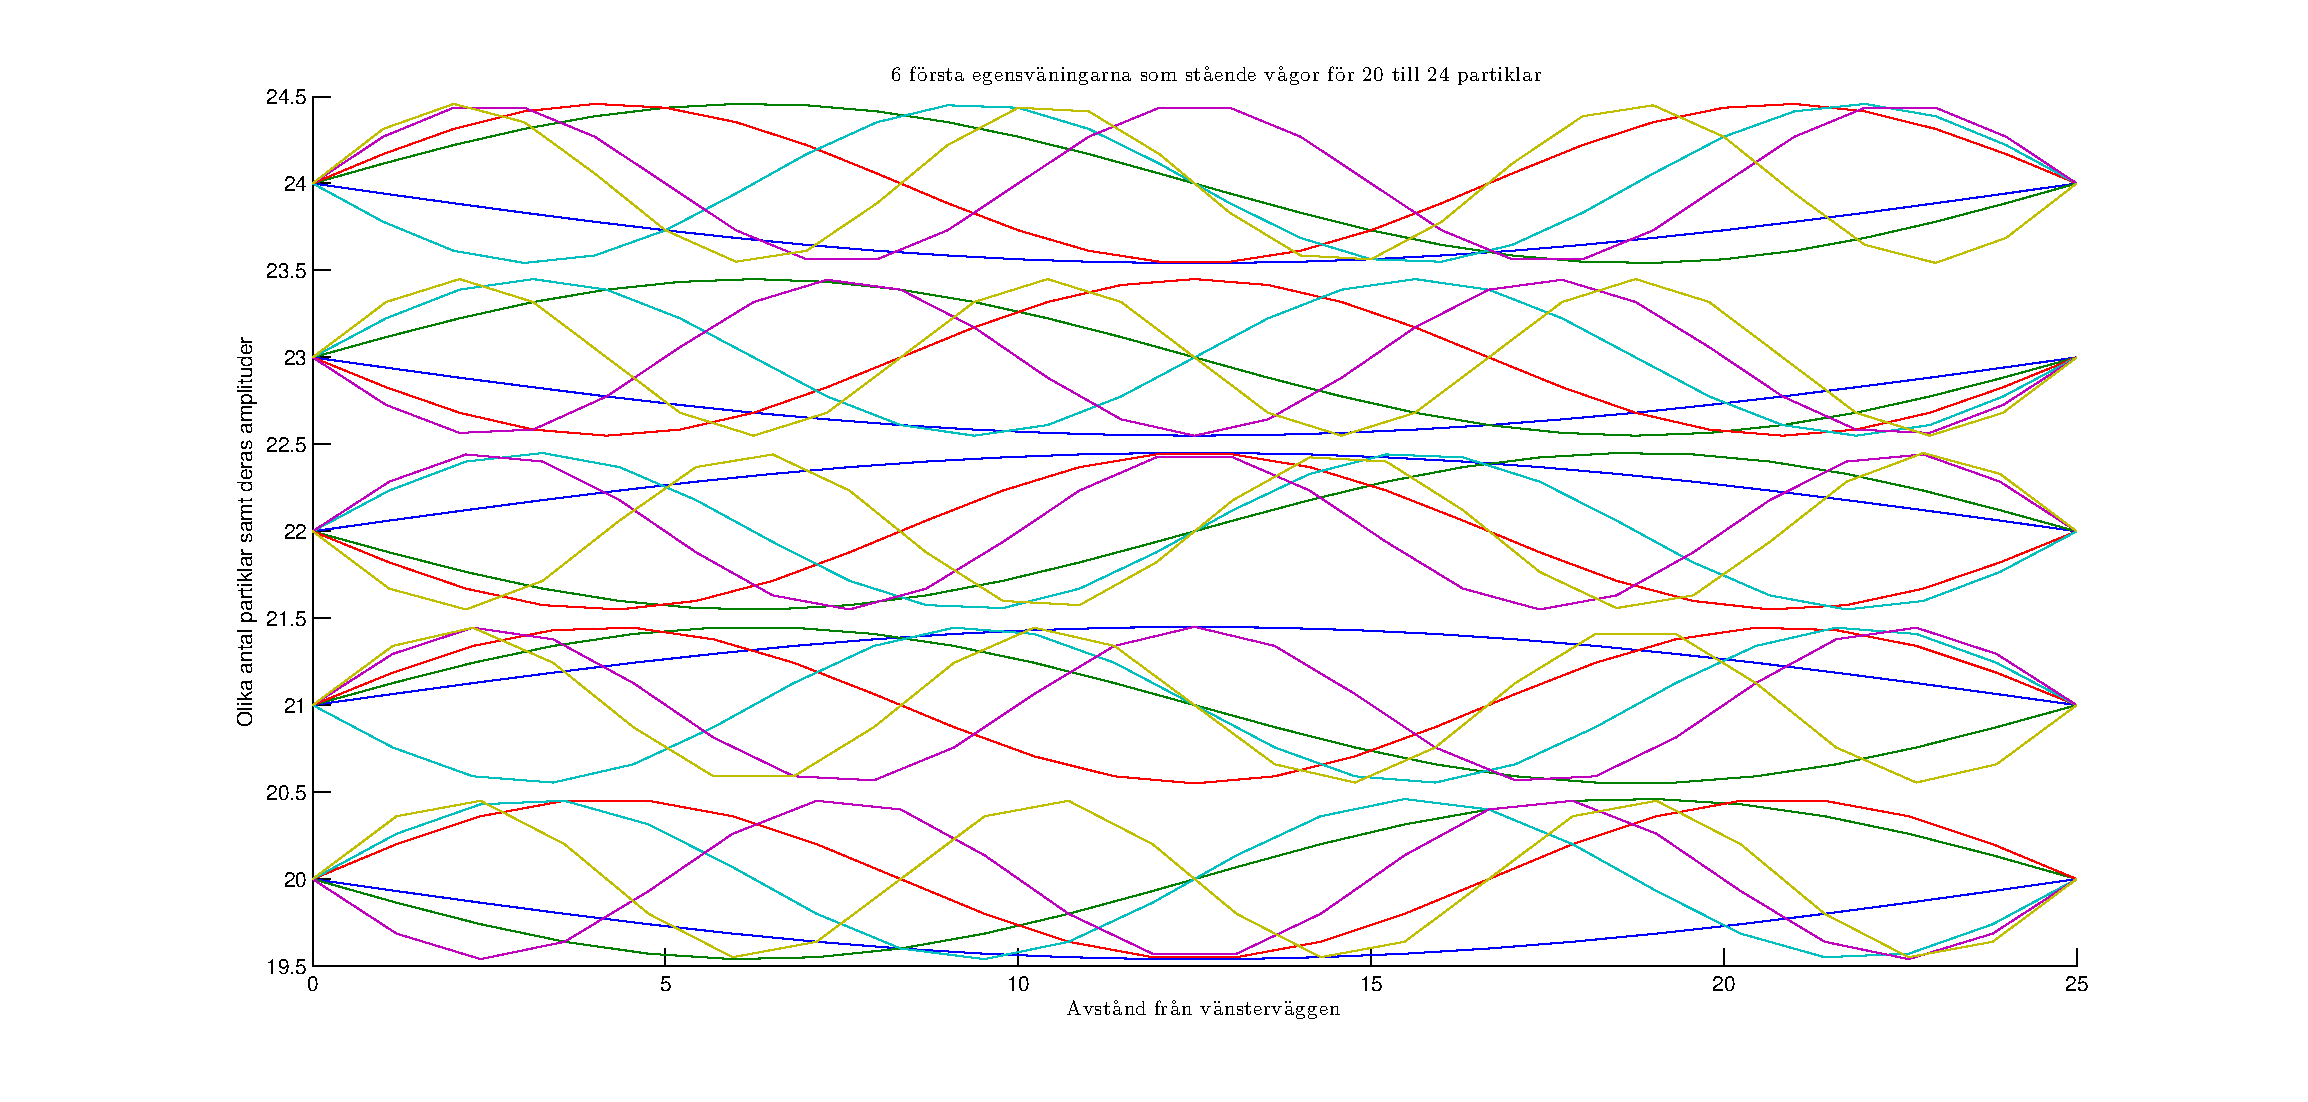
\includegraphics[width=\textwidth]{staendevagor.eps}
\end{figure}
\end{center}
		För att illustrera egenfrekvenserna så plottar vi sinusvågor med egenfrekvenserna.
		%bilder ska fixas, 10 till 20 partiklar verkar lämpligt, över 20 lär vara för svårtyt.
		\begin{center}
\begin{figure}
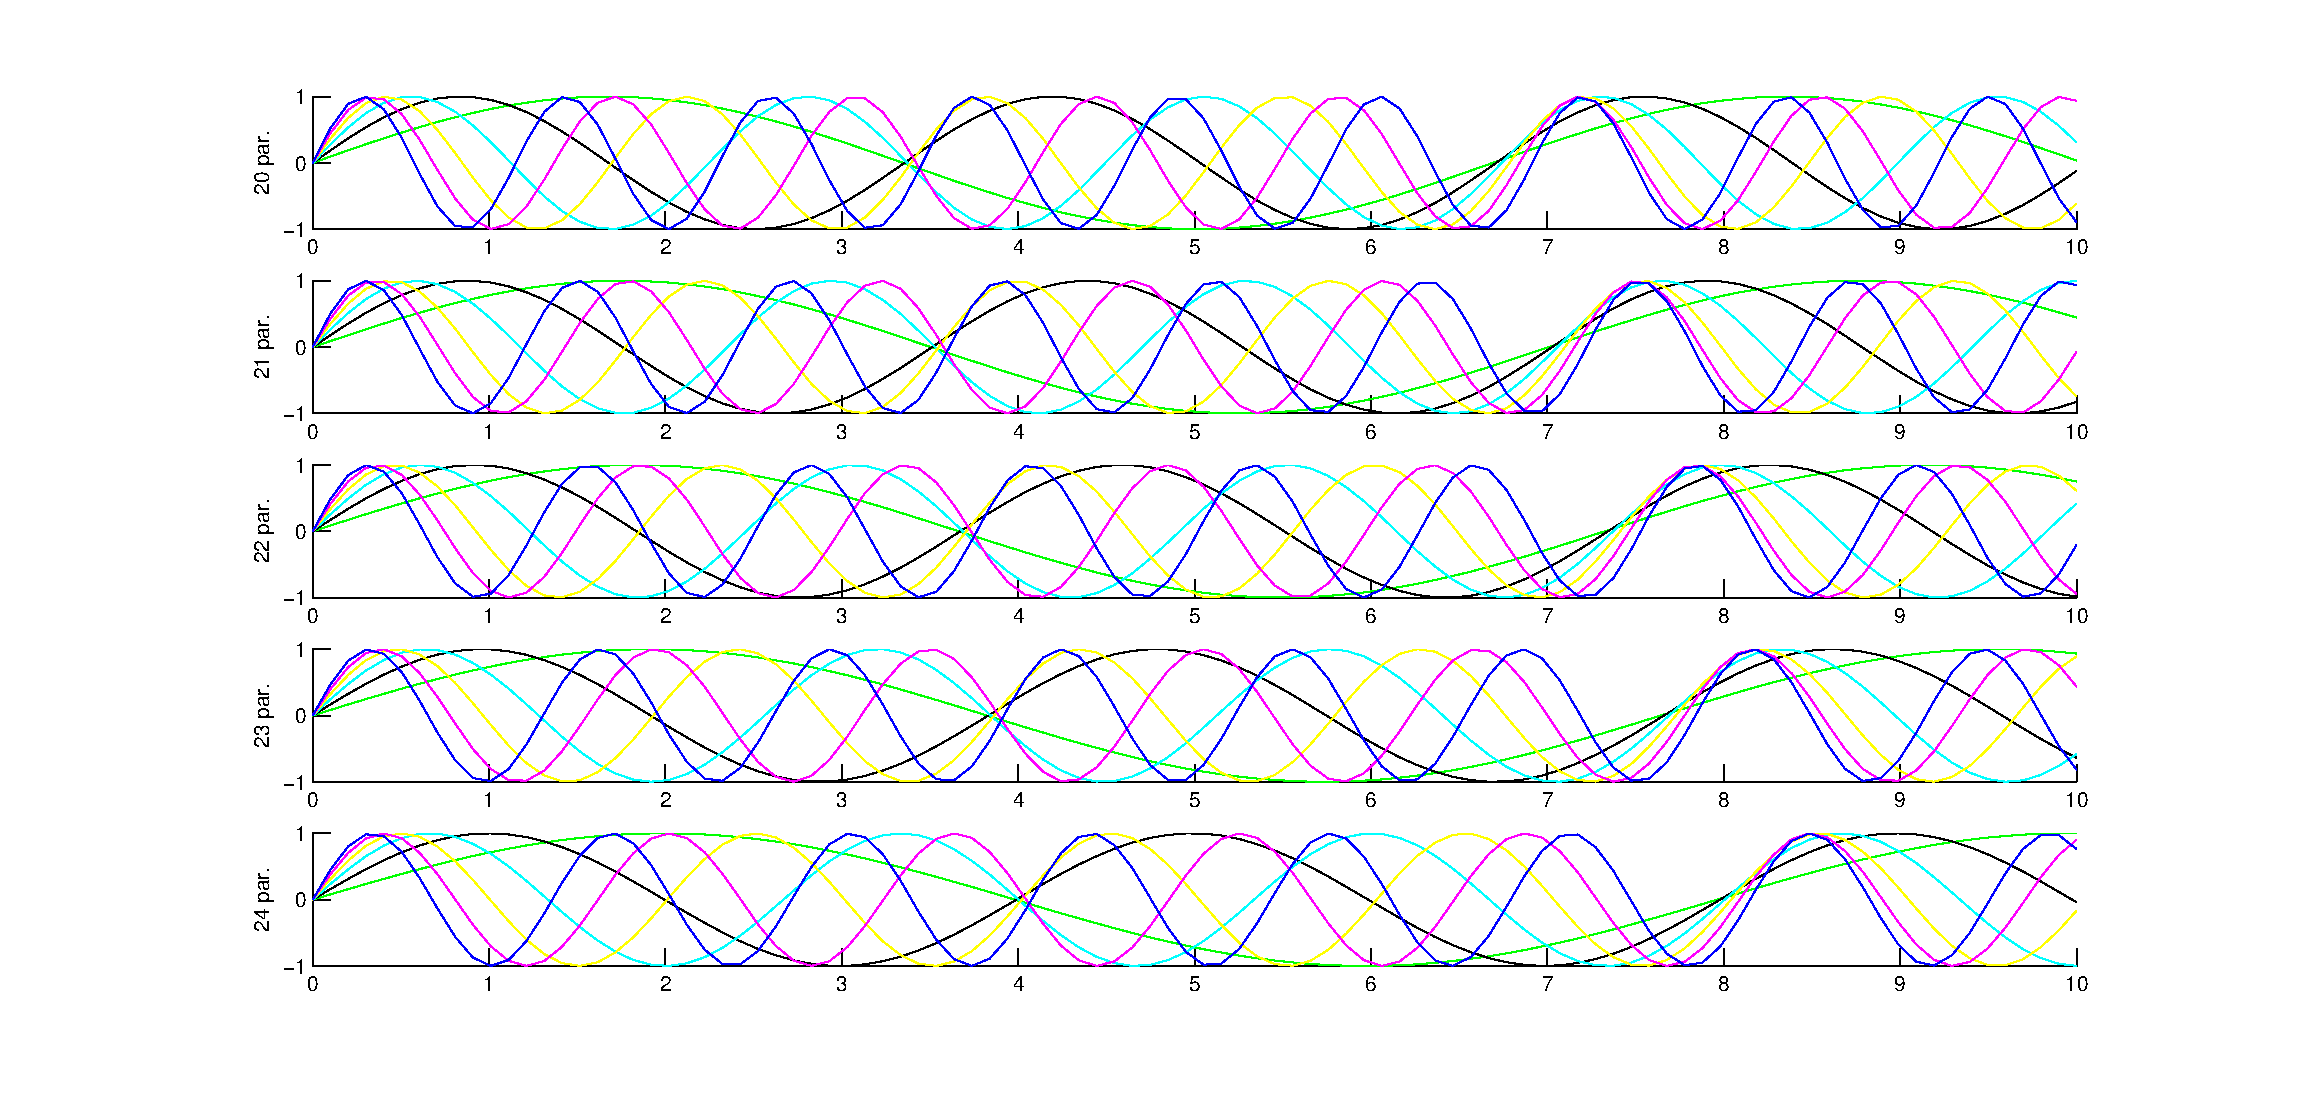
\includegraphics[width=\textwidth]{egenfrekvenser.eps}
\end{figure}
\end{center}
\end{document}
